\chapter{Results}

In this chapter, after we discussed the implementation of our method, we are going to check it after the assumptions we stated in TODO, discussing advantages, disadvantages, and trade-offs that was necessary to account for. In the first section, we will discuss the quality result of our method, comparing it to path-traced results. In the second section, we will discuss how close we can get to the expected results in the performance domain, seeing how well our implementation scales in different domains. 

\section{Parameters}
In this section, we are going to refer to some parameters of our method. The parameters were introduced in the previous chapter TODO. We will sum them up here, in order to have a reference for this chapter.

\begin{itemize}
\item $M$, the total number of points in the disk. We recall that we make a disc of the size of the object bounding box and then generate $M$ exponentially based samples in it. Unless otherwise stated, $M = 1000$
\item $q$, the modifier of the exponential distribution of the samples. So, the points are distributed on a circle with PDF $q \sigma_{tr}\exp(-q\sigma_{tr} r)$. Unless otherwise stated, $q = 1$. We choose $\sigma_{tr} = min(\sigma_{tr, red},\sigma_{tr, green},\sigma_{tr, blue})$, i.e. the minimum component spectrum wise.
\item $N$, the number of samples used from the disc. It is always $N < M$.
\item $K$, the number of directions used in the radiance map. Unless otherwise stated, $K = 16$. 
\item $L$, the number of lights in the scene. 
\item $W_l$, the size in pixel of the lightmaps. Unless otherwise stated, $W_l = 512$.
\item $W_r$, the size in pixel of the radiance map. Unless otherwise stated, $W_r = 1024$.
\end{itemize}


Other parameters are available in the method, such as all the parameters of the cameras. But even if we did not, those can be set up automatically. In this section, we listed only the parameters that makes sense for the user to tweak, and that can directly influence the quality or the performance of the final result.

\section{Quality comparison}

In the domain of quality, we compared our method to a solution obtain with a Monte Carlo path tracer that uses the directional dipole. The solutions are compared only visually, since if was not possible to perfectly match the perspective and view cameras of the original pictures. Thus, a RMSE comparison would not make sense.  We will see that the visual results of our method, given enough samples, can produce a result ofter comparable to the one of a path traced solution. We will compare our results at convergence (after 100 frames of evolution), to then also compare some of the results obtained during the evolution of the method. 

\subsection{Tests with different number of samples}

The material tested where potato, a highly scattering isotropic material ($\alpha = \sigma_s / \sigma_a \approx 10^2$), a even higher high scattering material, marble ($\alpha \approx 10^4$), a material with a big forward scattering component, white grapefruit juice ($\alpha \approx 10^2$, $g \approx 0.5$), ketchup a material that has a strong absorption component in the red channel ($\alpha_{red} \approx 10^{-2}$, $\alpha_{green} \approx \alpha_{blue} \approx 10^2$), and beer, a high absorption, forward scattering material with nearly no scattering. We are biased against highly scattering material because those are the material where our BSSRDF model gives our best results. However, we included materials as beer and ketchup to provide a comparison of our method even where the orgiginal BSSRDF model should fail.

The first comparison we make is with the path traced spheres generated in figure TODO. The results are illustrated in figure TODO, comparing different values of $M$ and $N$ for a potato sphere. We can see that different values of $M$ and $N$ greatly influence the results. In fact, for a big $M$ and the same $N$, the samples tend to be closer to the exitance point $x_o$, so the results is more accurate on the highlight region. If instead we chose a relatively small $M$, the points are more spread on the surface, to the absorption of the material is accounted more. This result in a sphere with gradients that are closer to the path trace solution. In this case, the highlights are way more difficult to see. 

The result that gets closer to the path traced solution is the one where $N = M = 1000$, but as we will see this values are unfeasible in the realm of performance, even for simple models. So, it is the artist that should find the right balance between $M$ and $N$ in order to get a satisfying result. 

In all cases, however, we observe a color shift to a greenish material compared to the path traced solution. Our guess is that the radius we are using is based on the minimum transmission coefficient $\sigma_{tr}$, that for potato is $\sigma_tr \approx (7, 14, 49) dm^{-1}$. So, the absorption is accounted more for the channels with the highest transmission coefficients (in this case, green and blue), that is probably causing the color shift. We will see that for materials with more homogenous scattering and absorption coefficients this phenomena is way more limited (as for example, in grapefruit juice and marble in figures TODO).

\begin{figure}
\centering
\subfloat[{$N = 120$, $M = 120$}]{
  \includegraphics[width=0.33 \linewidth]{images/results/test_120_over_120.png}
}
\subfloat[{$N = 120$, $M = 300$}]{
  \includegraphics[width=0.33 \linewidth]{images/results/test_120_over_300.png}
}
\subfloat[{$N = 300$, $M = 300$}]{
  \includegraphics[width=0.33 \linewidth]{images/results/test_300_over_300.png}
} \\
\subfloat[{$N = 120$, $M = 1000$}]{
  \includegraphics[width=0.33 \linewidth]{images/results/test_120_over_1000.png}
}
\subfloat[{$N = 300$, $M = 1000$}]{
  \includegraphics[width=0.33 \linewidth]{images/results/test_300_over_1000.png}
}
\subfloat[{$N = 1000$, $M = 1000$}]{
  \includegraphics[width=0.33 \linewidth]{images/results/test_1000_over_1000.png}
} \\
\subfloat[Path traced solution]{
  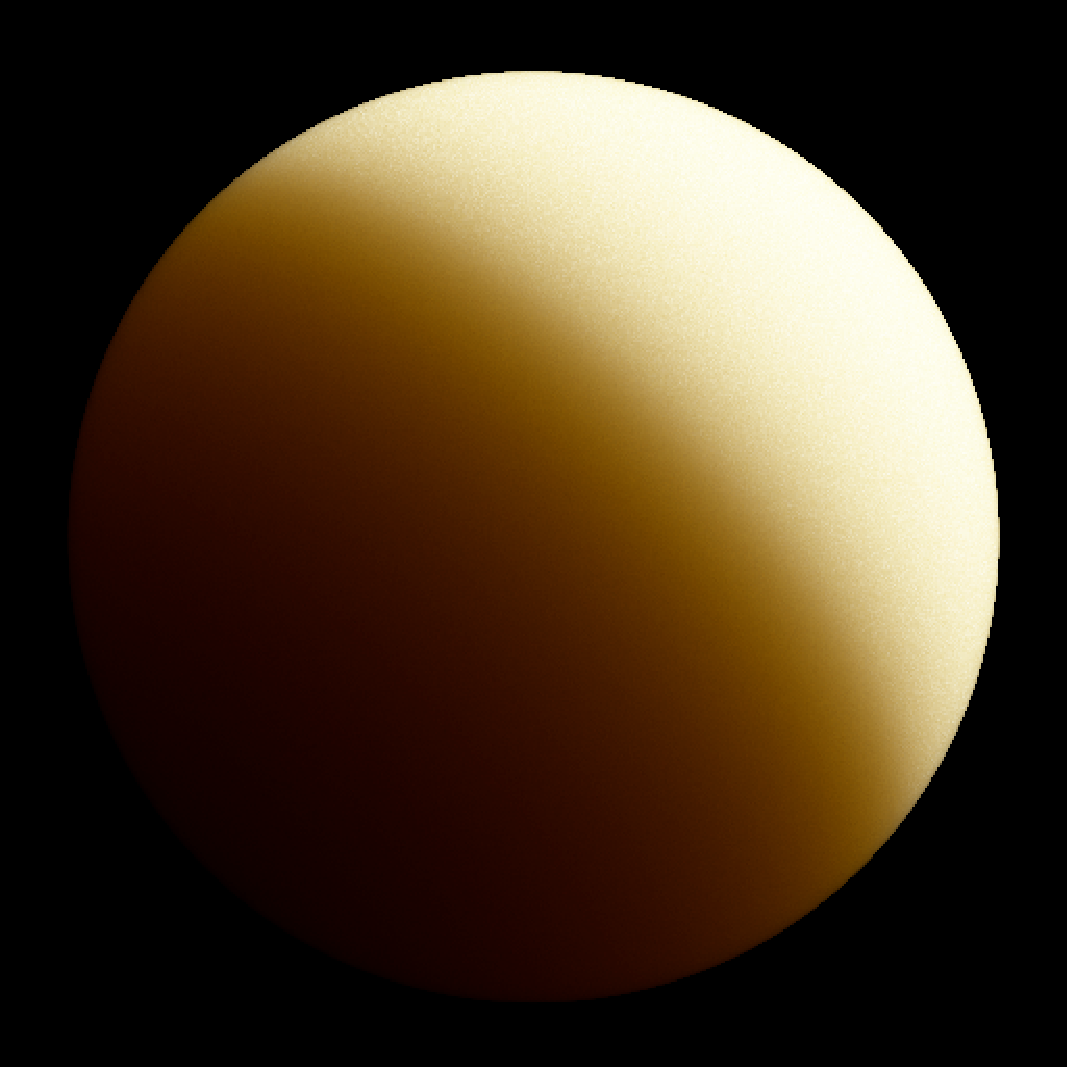
\includegraphics[width=0.33 \linewidth]{images/pathtrace/image-potato.pdf}
}
 \\
\label{fig:pathpotato}
\caption{Path traced rendering on a sphere of potato material compared with the results of our method. The parameters are from table \ref{table:scatteringcoefficients}.}
\end{figure}
 
In the next set of experiments, we can see the utility of the $q$ parameter. We tested a sphere of white grapefruit juice, a material with a high forward scattering component. In this case we can see that that with a smaller number of samples $N = 100$ and a $q = 3$ we can approximate very well the solution where $N = 1000$ and $q = 1$, way more expensive for the GPU. In a test with marble, in figure TODO we can see that our sampling introduces artifacts, especially on the color transition area. In this case, $q$ slightly relieves the artifacts generated from the sampling. Also in this case, our method does not capture the red color shift of the path traced solution, due to a higher blue scattering coefficient.

\begin{figure}
\centering
\subfloat[{$N = 100$, $M = 1000$, $q = 1$}]{
  \includegraphics[width=0.5 \linewidth]{images/results/grapefruit_juice_comparison_100_over_1000_nobias.png}
}
\subfloat[{$N = 100$, $M = 1000$, $q = 3$}]{
  \includegraphics[width=0.5 \linewidth]{images/results/grapefruit_juice_comparison_100_over_1000_bias3.png}
}
\\
\subfloat[{$N = 1000$, $M = 1000$, $q = 1$}]{
  \includegraphics[width=0.5 \linewidth]{images/results/grapefruit_juice_comparison.png}
}
\subfloat[{Path traced result}]{
  \includegraphics[width=0.5 \linewidth]{images/pathtrace/image-grapefruit.pdf}
}
\label{fig:pathgrapefruit}
\caption{Path traced rendering on a sphere of white grapefruit material compared with the results of our method. The parameters are from table \ref{table:scatteringcoefficients}. We can see that a higher $q$ helps us in approximating the path traced solution with fewer samples.}
\end{figure}

\begin{figure}
\centering
\subfloat[{$N = 120$, $M = 1000$, $q = 1.5$}]{
  \includegraphics[width=0.4 \linewidth]{images/results/marble_120_over_1000_bias_1-5.png}
}
\subfloat[{$N = 120$, $M = 1000$, $q = 1$}]{
  \includegraphics[width=0.4 \linewidth]{images/results/marble_120_over_1000_nobias.png}
}
\\
\subfloat[{$N = 1000$, $M = 1000$, $q = 1.5$}]{
  \includegraphics[width=0.4 \linewidth]{images/results/marble_1000_over_1000_bias_2.png}
}
\subfloat[{$N = 1000$, $M = 1000$, $q = 1$}]{
  \includegraphics[width=0.4 \linewidth]{images/results/marble_1000_over_1000_biasno.png}
}
\\
\subfloat[{Path traced result}]{
  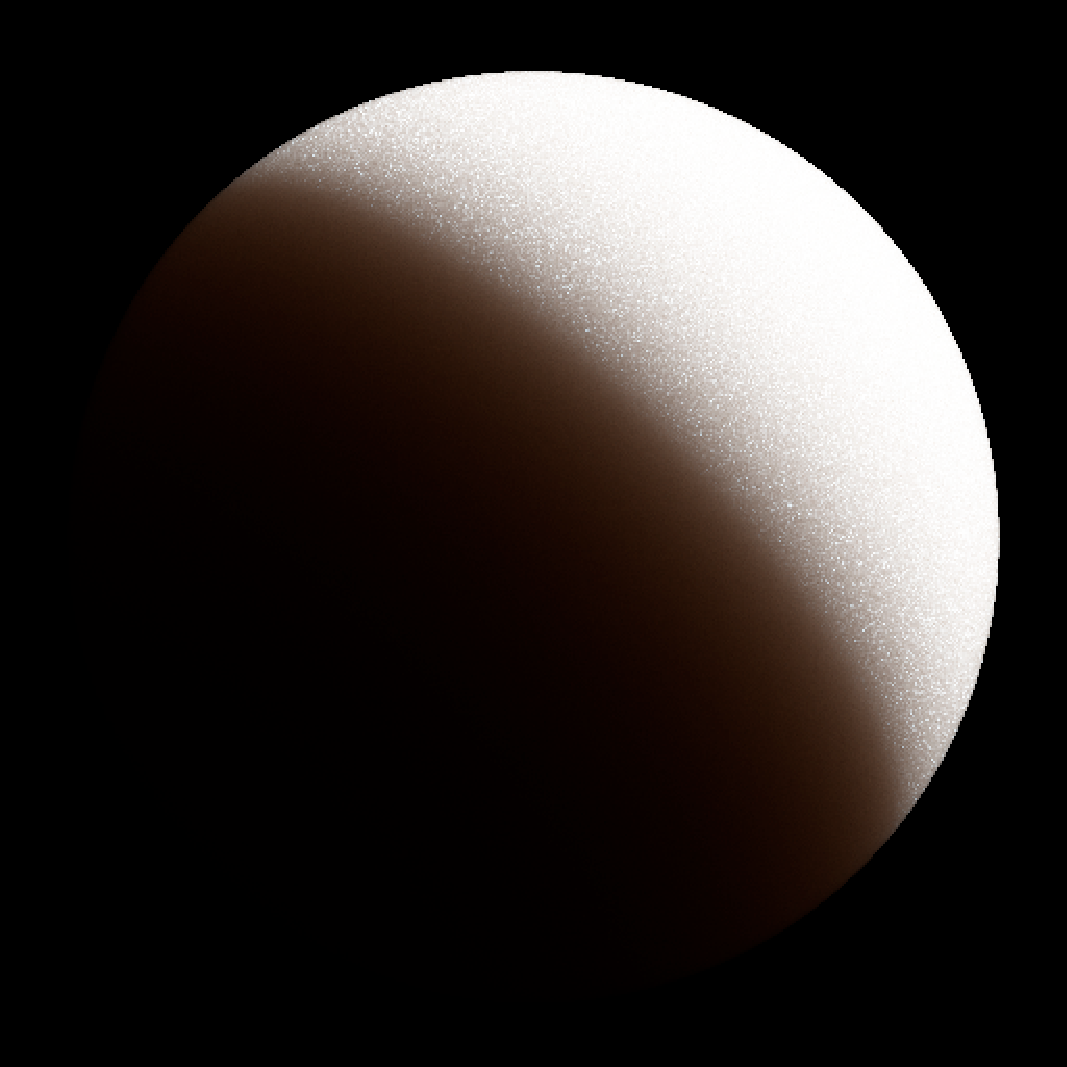
\includegraphics[width=0.4 \linewidth]{images/pathtrace/image-marble.pdf}
}
\label{fig:pathmarble}
\caption{Path traced rendering on a sphere of marble material compared with the results of our method. The parameters are from table \ref{table:scatteringcoefficients}.}
\end{figure}

\FloatBarrier
In figure TODO, we can see a comparison between our method and a beer material: despite the obvious artifacts due to sampling, our results show a more realistic result that a path traced one. This happens because of the extremely low scattering coefficient of beer, that makes it unfeasible to use a Monte Carlo path tracer, since we need to sum a lot of contribution in order to remove all the noise. 

\begin{figure}[!ht]
\centering
\subfloat[{$N = 100$, $M = 100$, $q = 1$}]{
  \includegraphics[width=0.5 \linewidth]{images/results/beer_100_over_100_no_bias.png}
}
\subfloat[{Path traced result}]{
  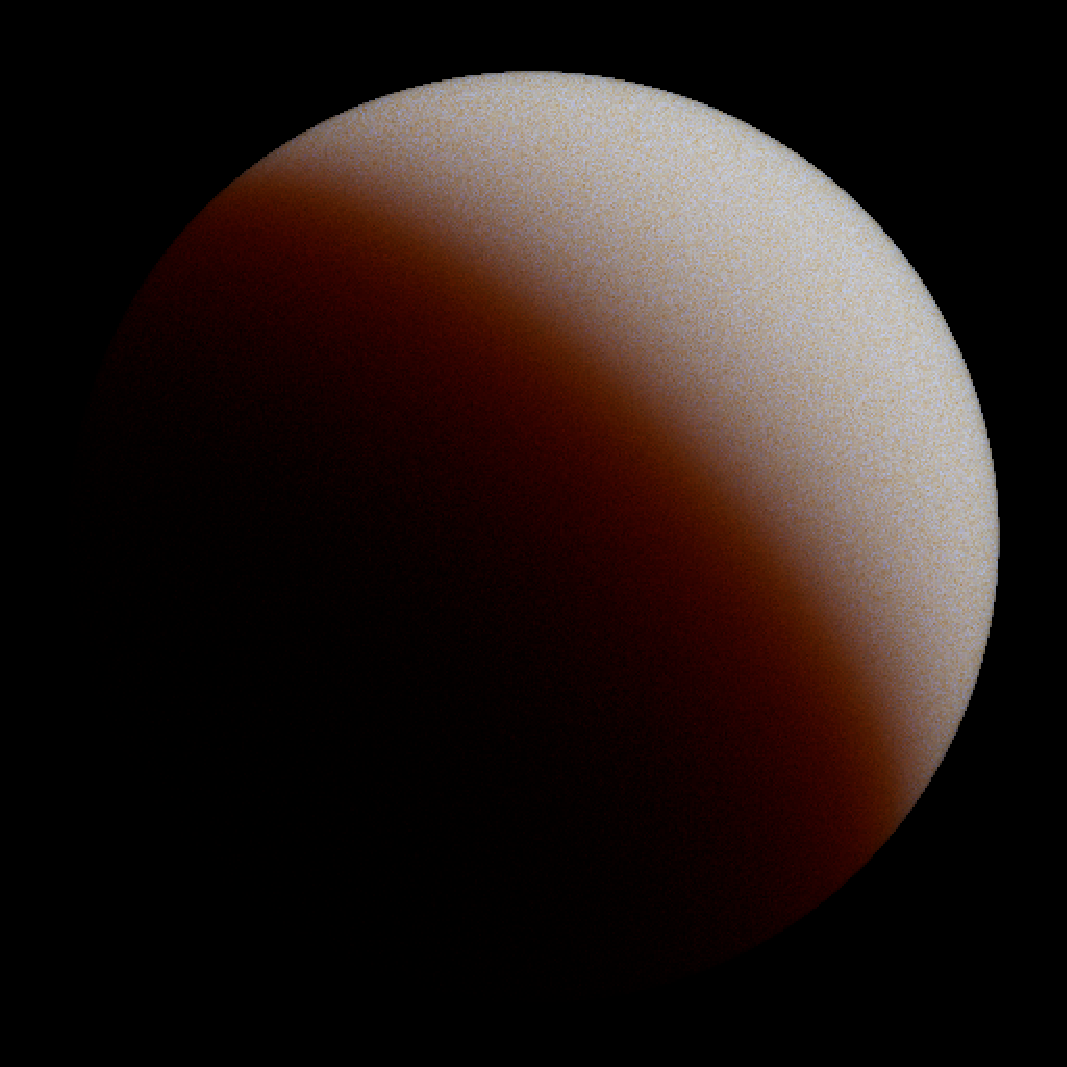
\includegraphics[width=0.5 \linewidth]{images/pathtrace/image-beer.pdf}
}
\label{fig:pathbeer}
\caption{Path traced rendering on a sphere of beer material compared with the results of our method. The parameters are from table \ref{table:scatteringcoefficients}.}
\end{figure}

The results that we obtained in the sphere renderings affect also the rendering of the full models. We tested a buddha made of potato, a dragon made of ketchup, and a bunny made of white grapefruit juice. We report here only the buddha and the dragon, while more results are available in appendix TODO. For the buddha, we observe a similar result (color shift) compared to reference as for the spheres in figure TODO.

For the ketchup dragon, instead, we observe that for a very low number of concentrated samples, the absorption contribution disappears, leaving only a gray scattering contribution that exhibits a pearling effect. If we reduce $M$, the highlights reduce and the absorption of red is accounted.


\begin{figure}
\centering
\subfloat[{$N = 100$, $M = 1000$, $q = 1$}]{
  \includegraphics[width=0.333 \linewidth]{images/results/happy_buddha_100_over_1000_nobias.png}
}
\subfloat[{$N = 200$, $M = 1000$, $q = 1$}]{
  \includegraphics[width=0.333 \linewidth]{images/results/happy_buddha_200_over_1000_nobias.png}
}
\subfloat[{Path traced result}]{
  \includegraphics[width=0.333 \linewidth]{images/results/potato_buddha_dir.png}
}
\label{fig:pathbuddha}
\caption{Rendering of a potato buddha using our method.}
\end{figure}


\begin{figure}
\centering
\subfloat[{$N = 10$, $M = 100$, $q = 1.5$}]{
  \includegraphics[width=0.5 \linewidth]{images/results/dragon_10_over_100.png}
}
\subfloat[{$N = 50$, $M = 120$, $q = 1$}]{
  \includegraphics[width=0.5 \linewidth]{images/results/dragon_50_over_120.png}
}
\\
\subfloat[{$N = 50$, $M = 1000$, $q = 1.5$}]{
  \includegraphics[width=0.5 \linewidth]{images/results/dragon_50_over_1000_nobias.png}
}
\subfloat[{Path traced result}]{
  \includegraphics[width=0.5 \linewidth]{images/results/ketchup_dragon_dir.png}
}
\label{fig:pathdragon}
\caption{TODO}
\end{figure}


\FloatBarrier

\subsection{Radiance map sizes tests}
Finally, we tested the effect of reducing the size of the texture used for the radiance map, for the dragon test. As we can see, for diminishing values of $W_s$ the quality does not get too much worse until $W_s = 128$, where artifacts due to shadow mapping become evident. In figure TODO the difference between the 1024 and the 256 image is reported. In the image, we can see that most of the difference are within $10\%$ of the high resolution value (since the image is enlarged 10 times and the full colored pixels are only a minority).

\begin{figure}
\centering
\subfloat[{$W_s = 128$}]{
  \includegraphics[width=0.5 \linewidth]{images/results/dragon_50_over_120_ws128.png}
}
\subfloat[{$W_s = 256$}]{
  \includegraphics[width=0.5 \linewidth]{images/results/dragon_50_over_120_ws256.png}
}
\\
\subfloat[{$W_s = 512$}]{
  \includegraphics[width=0.5 \linewidth]{images/results/dragon_50_over_120_ws512.png}
}
\subfloat[{$W_s = 1024$}]{
  \includegraphics[width=0.5 \linewidth]{images/results/dragon_50_over_120.png}
}
\label{fig:pathdragonsize}
\caption{TODO}
\end{figure}

\begin{figure}
\centering
  \includegraphics[width=1 \linewidth]{images/results/difference.png}
\label{fig:pathdragon}
\caption{Difference multiplied by 10 between TODO and TODO.}
\end{figure}

\FloatBarrier
\subsection{Tests of mipmap blurring quality}

In this part we tested the quality improvement from the mipmap blurring introduced in TODO to the final image. We can see the result of our method at the first frame and helfway though the simulation, as well as an adjusted mipmap level $m$. At the beginning of the evolution, a strong blurring is needed to compensate the high level noise, as we can see from image TODO. During the evolution, a lesser level of mipmaps is needed in order to preserve a noiseless image. At convergence, we do not need mipmap blurring at all. 

\begin{figure}
\centering
\subfloat[{Mipmap level 0 (no blur)}]{
  \includegraphics[width=0.4 \linewidth]{images/results/mipmaps00.png}
}
\subfloat[{Mipmap level 1}]{
  \includegraphics[width=0.4 \linewidth]{images/results/mipmaps01.png}
} \\

\subfloat[{Mipmap level 2}]{
  \includegraphics[width=0.4 \linewidth]{images/results/mipmaps02.png}
}
\subfloat[{Convergence}]{
  \includegraphics[width=0.4 \linewidth]{images/results/mipmapsc.png}
}
\label{fig:mipblurring}
\caption{Rendering of a potato dragon with different mipmap levels in the first frame of the computation, apart from the last one, that shows the result at convergence. We can see that the second mipmap level helps a lot in getting closer to the final result. However, some artifacts due to the stretching of the mipmap appear, such as black spot and bright seams. All the maps use the standard parameters, apart from $N = 32$ and $M = 300$.}
\end{figure}

\subsection{Environment map illumination}

All the given consideration so far are the same irregardless if we have an environment map or a single directional light. In this section we present the results obtained we environment light illumination. Visually, we obtain a nice result. Obviously, since the samples are split between different lights, an overlapping is inevitable, and we need an higher number of samples to obtain a decent result. The bunnies in figure TODO were obtained using 16 directional lights, sampled using the method in TODO and TODO, with $N = 80$ (5 samples per light) and $M = 1000$. 

As for reference, we compared our results to the reference image of the potato buddha presented in TODO. We had to try to match the light settings and the camera, but here as well we notice the same color shift as before. Also in this case we used 16 directional lights to represent our skybox.

\begin{figure}
\centering
\includegraphics[width=0.7 \linewidth]{images/results/bunny_env_80_1000_nobias.png}
\label{fig:bunnyenv1}
\caption{TODO}
\end{figure}

\begin{figure}
\centering
\subfloat[{Grace Cathedral}]{
  \includegraphics[width=0.5 \linewidth]{images/results/bunny_envgrace_80_1000_nobias.png}
}
\subfloat[{Pisa Courtyard}]{
  \includegraphics[width=0.5 \linewidth]{images/results/bunny_envPISA_80_1000_nobias.png}
}
\label{fig:bunnyenv}
\caption{TODO}
\end{figure}


\begin{figure}
\centering
\subfloat[{$L = 16$, $N = 90$, $M = 1000$}]{
  \includegraphics[width=0.333 \linewidth]{images/results/happy_buddha_environment_90over16_1000_nobias.png}
}
\subfloat[{$L = 16$, $N = 90$, $M = 300$}]{
  \includegraphics[width=0.333 \linewidth]{images/results/happy_buddha_environment_90over16_310_nobias.png}
}
\subfloat[{Path traced result}]{
  \includegraphics[width=0.333 \linewidth]{images/results/reference_env.png}
}
\label{fig:pathbuddhaenv}
\caption{Rendering of a potato buddha using our environment lighting and the Doge map.}
\end{figure}

\FloatBarrier

In the image of figure TODO, we compare the result using the Pisa Courtyard environment map on a Stanford Dragon, comparing a different number of lights. We can see the more lights we introduce, the more closer we get to a result that approximate true environment illumination. We observe also that the images have more scattering than absorption the more we increase the number of lights: this is because the total number of samples $N$ does not change, so each light has less and less samples available. In this way, the sampels tend to concentrate in thecenter and produce a result where the scatterign component is predominant.

\begin{figure}
\centering
\subfloat[{2 lights}]{
  \includegraphics[width=0.4 \linewidth]{images/results/env2.png}
}
\subfloat[{4 lights}]{
  \includegraphics[width=0.4 \linewidth]{images/results/env4.png}
} \\

\subfloat[{8 lights}]{
  \includegraphics[width=0.4 \linewidth]{images/results/env8.png}
}
\subfloat[{16 lights}]{
  \includegraphics[width=0.4 \linewidth]{images/results/env16.png}
}
\label{fig:mipblurring}
\caption{Rendering of a potato dragon ($N = 32$, $M = 300$) using a different number of directional light to represent the environment map.}
\end{figure}

\section{Performance comparisons}
In this section, we examine and analyze the performance of our method. 


\begin{table}[!ht]
\centering
\begin{tabular}{p{3cm}l|l|l|l|l|}
\cline{3-6}
                             &      & \multicolumn{4}{c|}{Number of samples ($N$)}                                          \\ \cline{3-6} 
                             & \#$\Delta$& \multicolumn{1}{c|}{1} & \multicolumn{1}{c|}{10} & \multicolumn{1}{c|}{50} & \multicolumn{1}{c|}{100} \\ \hline
\multicolumn{1}{|l|}{Bunny}  & $10^5$ & 4.1                  & 10.1                 & 21.4                  & 38.7                 \\ \hline
\multicolumn{1}{|l|}{Dragon} & $10^6$ & 13.9                 & 35.2                  & 139.6                & 270.8                \\ \hline
\multicolumn{1}{|l|}{Buddha} & $10^7$ & 91.5                 & 93.0                  & 121.4                & 209.2                 \\ \hline
\end{tabular}
\caption{Timings in milliseconds of our method for different models and number of samples $N$ (potato material properties). The other parameters were $L = 1$, $W_s = W_l = 512$, $M = 1000$, $q = 1$, $K = 16$.}
\end{table}



%TODO text and images